\section{Results}

Table \ref{tab:res_prost} shows the obtained DSCs for the segmentation of the prostate when the six trained models are used for the segmentation of the GE and Siemens dataset.  The displayed DSC is computed from the validation subset when the model is trained on the same dataset, and computed from the whole dataset when the model is trained from a different dataset. 
\begin{table}[h]
    \centering
    \begin{tabular}{|l|c|c|}
         \hline
          & \multicolumn{2}{c|}{ \textbf{Tested on} } \\
         \hline
          \textbf{Trained with} &  GE & Siemens  \\
         \hline
         GE: wo/w DA & 0.748/0.758 & 0.305/0.340 \\
         \hline
         Siemens: wo/w DA & \textbf{0.150}/0.310 & 0.898/0.889\\
         \hline
         GE \& Siemens: wo/w DA & 0.753/0.739 & 0.904/\textbf{0.915}\\
         \hline
    \end{tabular}
    \caption{Dice Similarity Coefficients between manual and CNN-generated prostate contours for GE and Siemens MRI vendors datasets. The trained models are divided in: with (w) data augmentation (DA) and without (wo) DA.}
    \label{tab:res_prost}
\end{table}
When the model is trained with examples from one dataset and used to segment prostates from scans of the same MRI vendor the average DSCs are: 0.753 for GE and 0.893 for Siemens. When the datasets are combined during training, the average DSC are: 0.746 for GE and 0.909 for Siemens.  The results obtained for the Siemens dataset are comparable with current state of the art methods for prostate segmentation. When the model is trained with examples from one MRI vendor and then used to process images from a different vendor, the resulting DSCs are low (0.322 and 0.169).  %This result exhibit 
The above shows how sensible the model is to subtle changes in the training dataset. It also displays the importance of testing how well deep learning architectures generalize to other MRI vendors.  The use of data augmentation improves the generalization of the models in most cases but not with a clear tendency, further analysis is required.

Table \ref{tab:res_pz} shows the obtained DSCs for the segmentation of the PZ the six trained models.  The best DSCs (0.653 and 0.756) for segmenting the PZ of the prostate are obtained when the model is trained using the combined dataset.  

\begin{table}[h]
    \centering
    \begin{tabular}{|l|c|c|}
         \hline
          & \multicolumn{2}{c|}{ \textbf{Tested on} } \\
        \hline
         \textbf{Trained with} &  GE & Siemens\\
         \hline
         GE: wo/w DA & 0.638/0.653& 0.331/\textbf{0.134} \\
         \hline
         Siemens: wo/w DA & 0.290/0.313 & 0.733/0.739\\
         \hline
         GE \& Siemens: wo/w DA & 0.648/0.654 & 0.743/\textbf{0.756}\\
         \hline
    \end{tabular}
    \caption{Dice Similarity Coefficients (DSC) between manual and CNN-generated PZ contours for GE and Siemens.The trained models are divided in: with (w) data augmentation (DA) and without (wo) DA.}
    \label{tab:res_pz}
\end{table}

The average DSCs of all the PZ models are lower than the coefficients for segmenting the prostate, which implies that PZ segmentation is a more challenging task.

Figure \ref{fig:resseg} shows one example of a prosate segmentation on the Siemens MRI vendor and a PZ segmentation on the GE MRI vendor. Both examples are from the middle layer of the prostate, and their corresponding DSC are 0.903 and 0.737.
\begin{figure}[h]
    \centering
    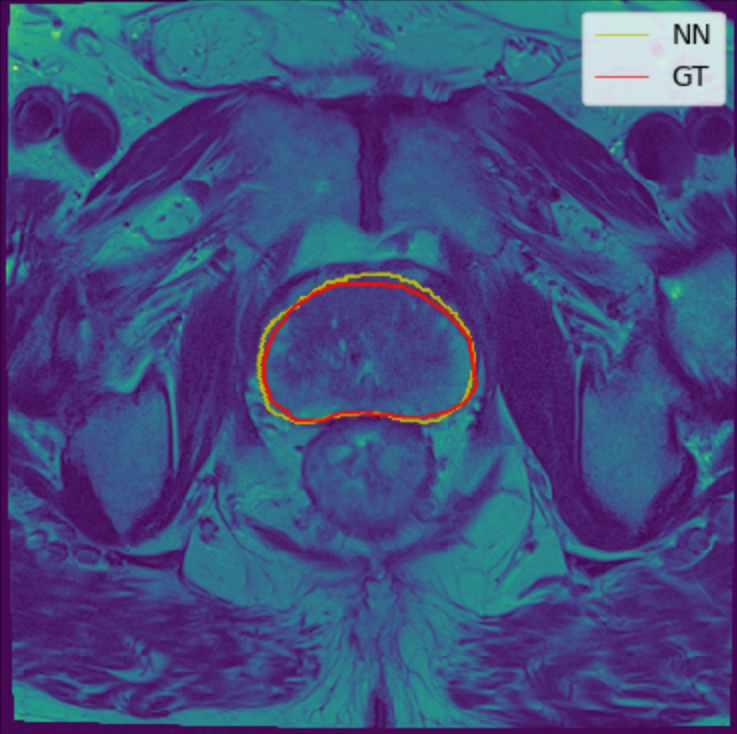
\includegraphics[totalheight=.18\textheight]{imgs/results/prosate.png}
    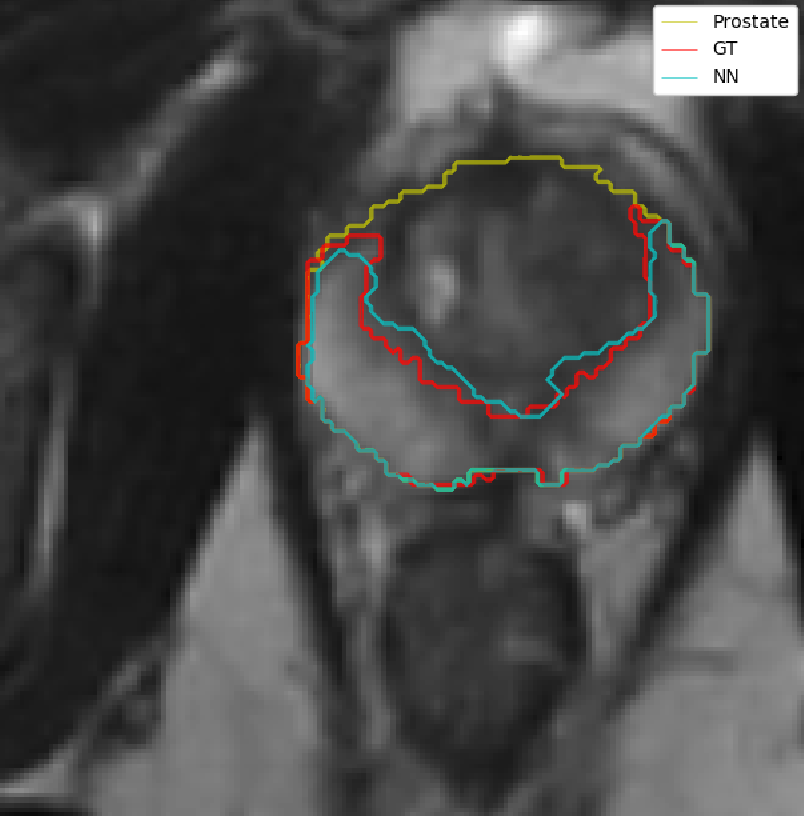
\includegraphics[totalheight=.18\textheight]{imgs/results/pz.png}
    \caption{Segmentation example of prostate (left) and peripheral zone (right) on Siemens and GE MRI vendors respectively. The obtained DSCs for these examples are 0.903 for the prostate and 0.737 for the peripheral zone.}
    \label{fig:resseg}
\end{figure}
